\documentclass[../nirs.tex]{subfiles}

\begin{document}
\section{Теоретическое изучение предметной области. Построение теоретических
математических моделей}

Система ТО создает нормативную базу технической эксплуатации автомобилей
(ТЭА) и определяет технологию и организацию проведения работ по ТО для
обеспечения заданных показателей качества автомобиля в процессе эксплуатации. К
системе ТО предъявляется ряд требований, главные из которых сводятся к
следующему:
\begin{itemize}
    \item обеспечение заданных уровней эксплуатационной надежности автомобилей
        при рациональных материальных и трудовых затратах;
    \item ресурсосберегающая и экологическая направленность;
    \item планово-нормативный характер, позволяющий планировать и организовывать
        ТО на всех уровнях управления, начиная от автотранспортных
        предприятий (АТП) до общегосударственных плановых и директивных органов;
    \item обязательность в смысле соблюдения принципов и нормативов для всех
        организаций и предприятий, владеющих автомобильным транспортом, вне
        зависимости от их ведомственного подчинения;
    \item конкретность, доступность и пригодность для руководства и принятия
        решений всеми звеньями интеллектуальной транспортной системы (ИТС);
    \item стабильность основных принципов, гибкость организационных методов
        реализации этих принципов и нормативов, позволяющих развивать инициативу
        персонала и учитывающих изменение условий эксплуатации, качества и
        надежности автомобилей, квалификацию и заинтересованность персонала, а
        также организационной структуры;
    \item количественный учет разнообразия условий эксплуатации подвижного
        состава, позволяющий объективно сравнивать и планировать результаты
        деятельности отдельных АТП, управлений и объединений с учетом реальных
        условий работы и имеющихся ресурсов.
\end{itemize}

Система ТО занимает важное место в концепции управления качеством
автомобилей. Сфера эксплуатации влияет на следующие реализуемые показатели
качества:
\begin{itemize}
    \item интенсивность изменения показателя качества;
    \item срок службы;
    \item начальные показатели качества.
\end{itemize}

Система ТО оказывает существенное влияние на реализуемые показатели качества
изделия и эффективность самой технической эксплуатации; определяет стратегию
обеспечения работоспособности автомобильного парка; создают нормативную базу,
обеспечивающую принятие рациональных технологических, проектных и
организационных решений, и условия для контроля качества технологических
процессов; определяет и нормирует необходимые ресурсы для технического
обеспечения транспортного процесса.

По данным исследований удовлетворительное выполнение рекомендаций системы ТО
обеспечивает в среднем повышение коэффициента технической готовности на 2,5 --
3\%, наработок на отказы и неисправности по различным узлам и механизмам в 1,2
-- 1,9 раз, сокращение расхода топлива на 1,5 -- 3,0\%.

Применяемые системы технического обслуживания массовых изделий
базируются на определенных стратегиях обеспечения работоспособности. Всю
возможную совокупность наиболее типичных отказов и неисправностей автомобиля
(400-700 в зависимости от конструкции и условий работы) можно подразделить на
две большие группы: профилактируемые и непрофилактируемые. К последним
относятся, во-первых, отказы и неисправности, которые невозможно заранее
предвидеть у конкретного автомобиля, т.е. внезапные; во-вторых, отказы и
неисправности, которые нецелесообразно предотвращать по экономическим или иным
критериям. Таких отказов и неисправностей у современных автомобилей около
27-39\% от общего числа. Для них действует стратегия \rom{2} (рисунок
\ref{fig:pdf.a}), заключающаяся в том, что они устраняются по мере
возникновения, т.е. по потребности. Иногда ее называют \textquote{стратегией
ожидания ремонта}. Если в качестве целевой функции принять затраты, то для
стратегии \rom{2} удельные затраты на ремонт:

\begin{equation*}
    C^{\rom{2}} =
    c\,/\,\bar{x} =
    c : \int_{x_{min}}^{x_{max}} x f(x)\,dx,
\end{equation*}
где $\bar{x},\,x_{min} \,\text{и} \,x_{max}$ -- соответственно средняя,
минимальная и максимальная наработки на отказ; $c$ -- разовые затраты на
устранение отказа; $f(x)$ -- плотность вероятности наработки на отказ.

\begin{figure}[H]
\centering
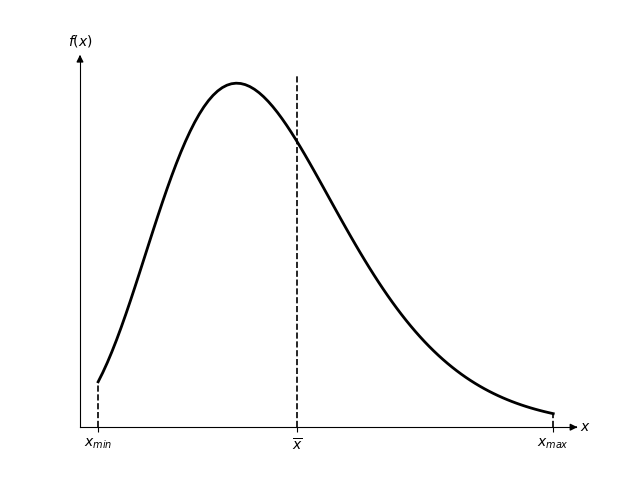
\includegraphics[keepaspectratio,width=\textwidth]{./images/pdf.a.png}
\caption{Стратегия обеспечения работоспособности. Устранения отказов по
    потребности}
\label{fig:pdf.a}
\end{figure}

Преимуществом стратегии \rom{2} является простота реализации, основным
недостатком -- неопределенность состояния конкретного изделия, которое может
отказать в любое время, а также трудность планирования и организации
технического обслуживания парка.

Для профилактируемой группы отказов и неисправностей может применяться как
стратегия поддержания (проведение технического обслуживания), так и стратегия
восстановления (ремонт) работоспособности. Выделение из этой группы
профилактируемых отказов и неисправностей производится исходя из заданных
критериев эффективности, например обеспечения необходимых уровней безопасности
движения, минимизации затрат ТО, повышения уровня работоспособности,
сокращения расхода топлива и т.д., причем критерии эффективности могут меняться
исходя из конкретных условий и ограничений.

Стратегия \rom{1} -- профилактическая, предусматривает предупреждение
значительной доли отказов и неисправностей данного наименования, восстановление
исходного или близкого к нему технического состояния изделия до того, как будет
достигнуто предельное состояние. Поэтому разовые затраты на одно воздействие на
поддержание работоспособности по стратегии \rom{1} ($d_{\text{п}}$), как правило
значительно ниже соответствующих затрат стратегии \rom{2} ($c$), т.е. $c \gg
d_{\text{п}}$, что и является основным источником эффективности профилактической
стратегии. Эта стратегия реализуется при предупредительном техническом
обслуживании, диагностике, предупредительных заменах некоторых деталей, узлов,
механизмов и т.д. При стратегии \rom{1} устанавливается наработка (периодичность
ТО), при которой изделию восстанавливают исходное или близкое к нему техническое
состояние (рисунок \ref{fig:pdf.b}).

\begin{figure}[H]
\centering
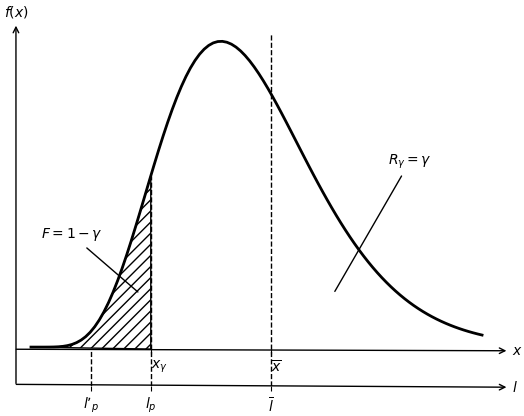
\includegraphics[keepaspectratio,width=\textwidth]{./images/pdf.b.png}
\caption{Стратегия обеспечения работоспособности. Предупреждение отказов
    (поддержание работоспособности по наработке)}
\label{fig:pdf.b}
\end{figure}

Применяются два основных метода реализации стратегии \rom{1}: планирование
воздействий по наработке с доведением параметра технического состояния до нормы
(\rom{1} -- 1, рисунок \ref{fig:pdf.b}); планирование контроля параметра
технического состояния по наработке с доведением до нормы в зависимости от
фактического и допустимого значений параметра технического состояния (\rom{1} --
2, рисунок \ref{fig:pdf.c}). Поэтому при стратегии \rom{1} профилактическая
операция в общем виде состоит из двух частей -- контрольной и исполнительской:
\begin{equation*}
    d_{\text{п}} = d_{\text{к}} + k d_{\text{и}}\,,
\end{equation*}
где $d_{\text{п}}$ -- стоимость ТО (профилактики); $d_{\text{к}}$ -- стоимость
контрольно-диагностической части операции ТО; $k$ -- коэффициент повторяемости
исполнительской части операции ТО; $d_{\text{и}}$ -- стоимость исполнительской
части операции ТО [\ref{ref:кузнецов}, стр. 170].

\begin{figure}[H]
\centering
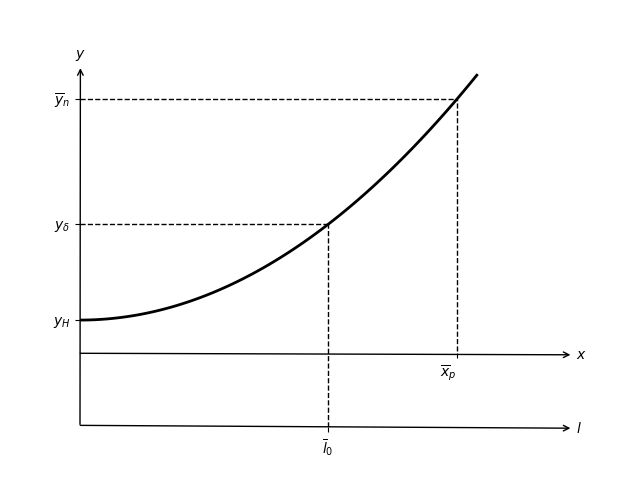
\includegraphics[keepaspectratio,width=\textwidth]{./images/pdf.c.png}
\caption{Стратегия обеспечения работоспособности. Предупреждение отказов
    (поддержание работоспособности по наработке)}
\label{fig:pdf.c}
\end{figure}


\end{document}
